\documentclass[tikz,border=8pt]{standalone}
\usepackage{helvet}
\renewcommand{\familydefault}{\sfdefault}
\usetikzlibrary{arrows.meta,positioning,shapes.geometric}
\begin{document}
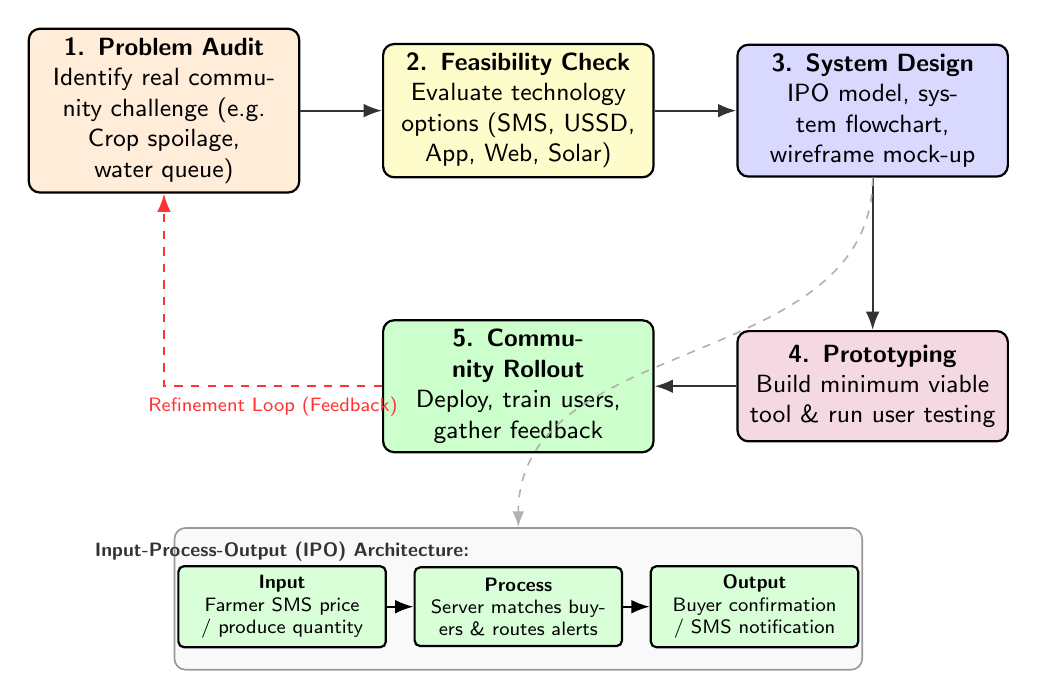
\begin{tikzpicture}[
    line width=0.8pt, 
    font=\sffamily\small, 
    >=Latex,
    stage/.style={rectangle, rounded corners=4pt, draw=black, fill=blue!10, text width=3.2cm, minimum height=1.4cm, align=center, line width=0.8pt},
    ipo/.style={rectangle, rounded corners=2pt, draw=black, fill=green!15, text width=2.4cm, minimum height=1.0cm, align=center, font=\sffamily\scriptsize},
    arrow/.style={->, thick, draw=black!80}
]

% ---- Stages -----------------------------------------------------------------
\node[stage, fill=orange!15] (s1) at (0,6.0) {\textbf{1. Problem Audit}\\Identify real community challenge (e.g. Crop spoilage, water queue)};
\node[stage, fill=yellow!20] (s2) at (4.5,6.0) {\textbf{2. Feasibility Check}\\Evaluate technology options (SMS, USSD, App, Web, Solar)};
\node[stage, fill=blue!15] (s3) at (9.0,6.0) {\textbf{3. System Design}\\IPO model, system flowchart, wireframe mock-up};

\node[stage, fill=purple!15] (s4) at (9.0,2.5) {\textbf{4. Prototyping}\\Build minimum viable tool \& run user testing};
\node[stage, fill=green!20] (s5) at (4.5,2.5) {\textbf{5. Community Rollout}\\Deploy, train users, gather feedback};

% ---- Stage Arrows -----------------------------------------------------------
\draw[arrow] (s1) -- (s2);
\draw[arrow] (s2) -- (s3);
\draw[arrow] (s3) -- (s4);
\draw[arrow] (s4) -- (s5);
\draw[arrow, dashed, red!80] (s5) -| (s1) node[pos=0.25, below, font=\sffamily\scriptsize, text=red!80] {Refinement Loop (Feedback)};

% ---- Detailed IPO Box below Stage 3 -----------------------------------------
\node[draw=gray!80, fill=gray!5, rounded corners=4pt, line width=0.6pt, text width=8.5cm, minimum height=1.8cm] (ipobox) at (4.5,-0.2) {};
\node[font=\sffamily\scriptsize\bfseries, text=black!80] at (1.5,0.4) {Input-Process-Output (IPO) Architecture:};

\node[ipo] (in) at (1.5,-0.3) {\textbf{Input}\\Farmer SMS price / produce quantity};
\node[ipo] (proc) at (4.5,-0.3) {\textbf{Process}\\Server matches buyers \& routes alerts};
\node[ipo] (out) at (7.5,-0.3) {\textbf{Output}\\Buyer confirmation / SMS notification};

\draw[->, thick] (in) -- (proc);
\draw[->, thick] (proc) -- (out);

\draw[->, gray!60, line width=0.6pt, dashed] (s3.south) to [out=270, in=90] (ipobox.north);

\end{tikzpicture}
\end{document}
